%%
%% This is file `mcmthesis-demo.tex',
%% generated with the docstrip utility.
%%
%% The original source files were:
%%
%% mcmthesis.dtx  (with options: `demo')
%% 
%% -----------------------------------
%% 
%% This is a generated file.
%% 
%% Copyright (C)
%%     2010 -- 2015 by Zhaoli Wang
%%     2014 -- 2016 by Liam Huang
%% 
%% This work may be distributed and/or modified under the
%% conditions of the LaTeX Project Public License, either version 1.3
%% of this license or (at your option) any later version.
%% The latest version of this license is in
%%   http://www.latex-project.org/lppl.txt
%% and version 1.3 or later is part of all distributions of LaTeX
%% version 2005/12/01 or later.
%% 
%% This work has the LPPL maintenance status `maintained'.
%% 
%% The Current Maintainer of this work is Liam Huang.
%% 
\documentclass{mcmthesis}

\mcmsetup{CTeX = false,   % 使用 CTeX 套装时,设置为 true
        tcn = {Yucheng Jin, Heyuan Li}, problem = A,
        sheet = true, titleinsheet = true, keywordsinsheet = true,
        titlepage = false, abstract = false}
\usepackage{gensymb}
\usepackage{graphicx,float}
\usepackage{palatino}
\usepackage[stable]{footmisc}
\usepackage{lipsum}
\usepackage{booktabs,siunitx}
\usepackage{amsthm}
\usepackage{lastpage}
\usepackage{fancyhdr}
\usepackage{array}
\usepackage{setspace}
\usepackage{textcomp}
\cfoot{\thepage}
\title{When "Spring" Comes to North Atlantic}

\begin{document}



\begin{center}


\item
\item

\huge{ECE 498 ICC} 

\huge{SP 2020}



\Large{Prof. V. Kindratenko}

\end{center}

\begin{center}

\item
\item
\item
\Huge{Lab 2 Report}



\Huge{Enabling Edge AI in Raspberry Pi}

\end{center}

\begin{center}

\item
\item
\item
\Large{Name: Yucheng Jin}
\item
\Large{ID: \qquad 3170112253}
\item
\Large{Name: \text{ } Heyuan Li}
\item
\Large{ID: \qquad 3160103193}
\item
\Large{Date: \text{ } April 19, 2020}


\end{center}

\pagebreak
\renewcommand{\contentsname}{\tiny{}}
\begin{center}
\textbf{\Large{Table of Contents}}
\end{center}
\tableofcontents
\pagebreak

\section{Part I}
\subsection{Check Point I}
\textbf{[1 pts]} Properly label all nodes within the Remote GPU service (by changing the name fields in their properties panel) and include a screenshot of the Remote GPU service subflow.
\begin{center}
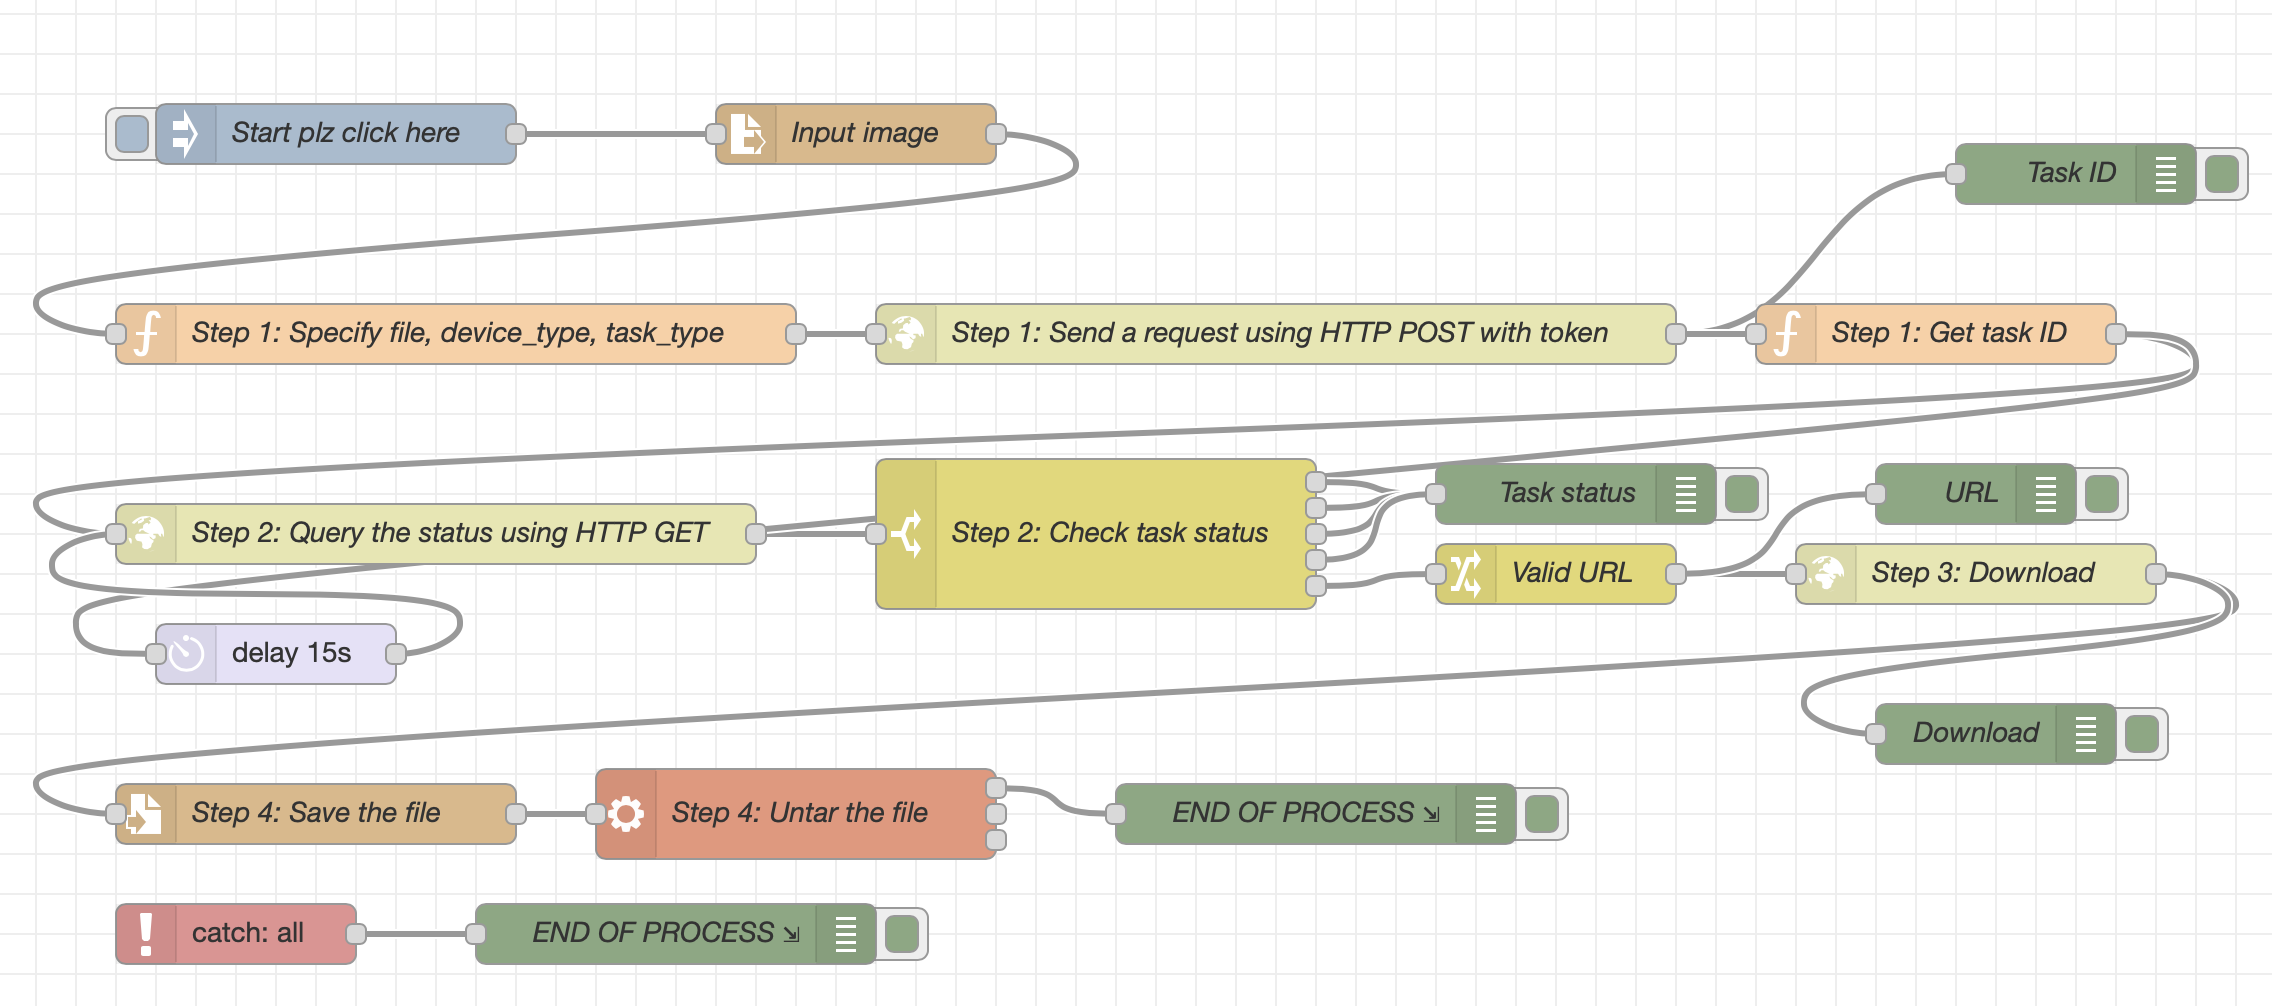
\includegraphics[width=15cm]{part1.png}
\end{center}

Above is our remote GPU service flow for Part I.

\subsection{Check Point II}
\textbf{[2 pts]} According to steps listed in the implementation checklist, divide nodes within the Remote GPU service into groups for achieving diferent goals and comment on each of these groups to justify that your design meet our requirements.
\begin{itemize}
\item \textbf{Input image}
\begin{center}
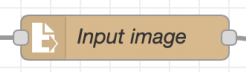
\includegraphics[width=5cm]{1.png}
\end{center}
This node is a \textit{file in} node which inputs the image file.
\begin{center}
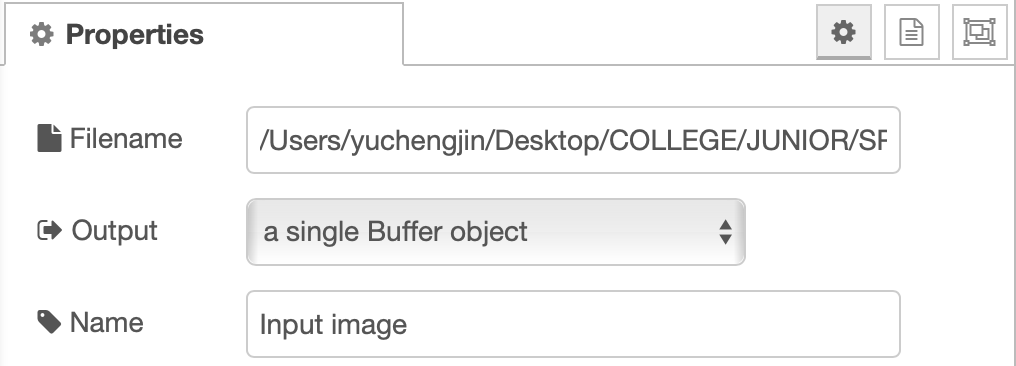
\includegraphics[width=12cm]{1_1.png}
\end{center}
\item \textbf{Step 1}
\begin{center}
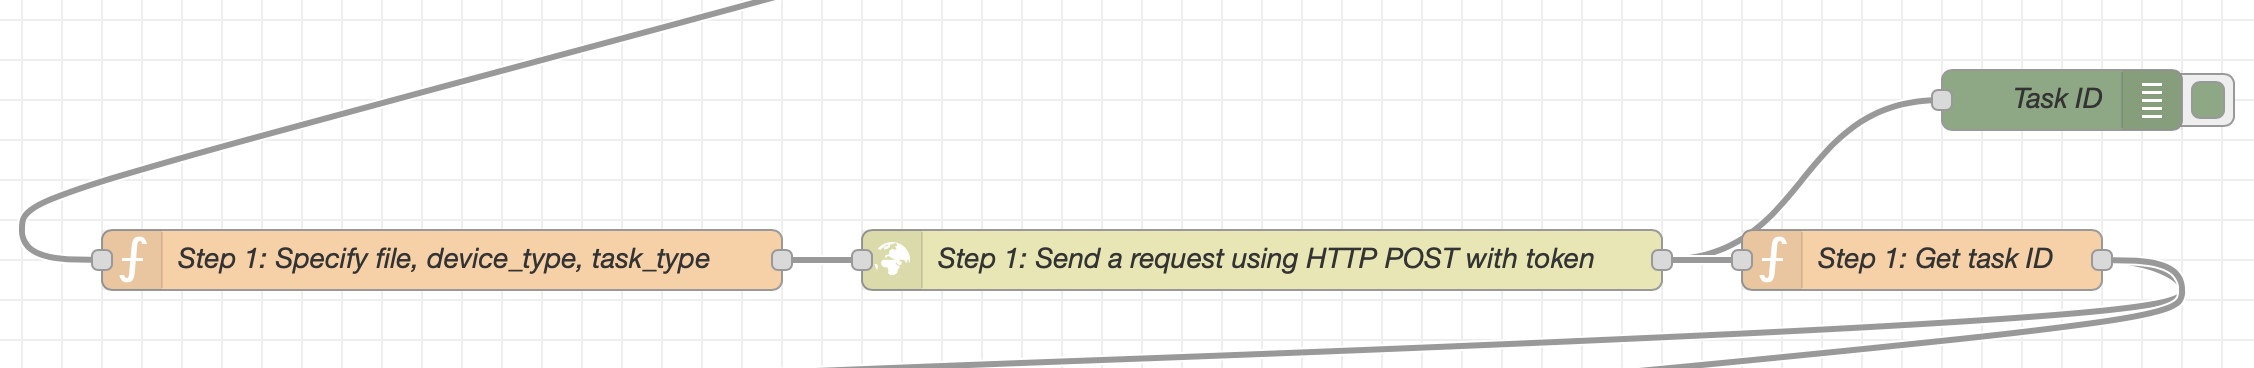
\includegraphics[width=12cm]{2.png}
\end{center}
There are 4 nodes in this group, including a \textit{function} node which specifies data type, key name for the file, device type, and task type,
\begin{center}
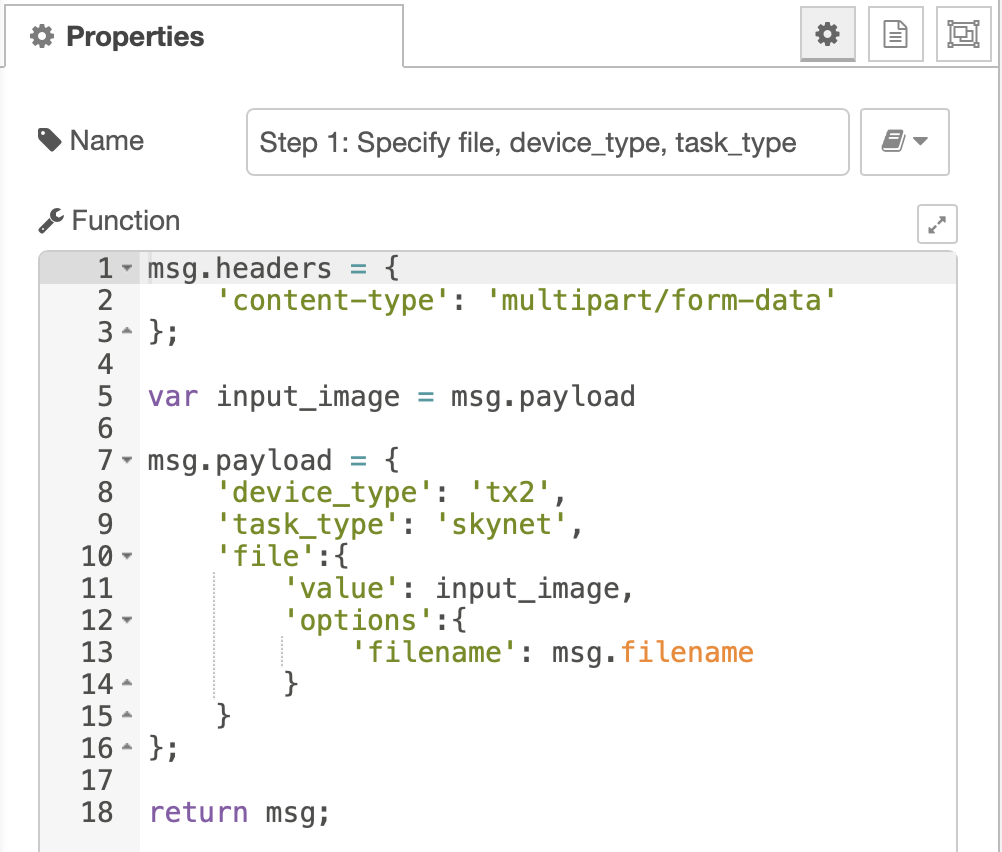
\includegraphics[width=12cm]{2_1.png}
\end{center}
an \textit{HTTP request} node which sends a request to http://141.142.204.78/uploader authorized with the token generated by pyjwt,
\begin{center}
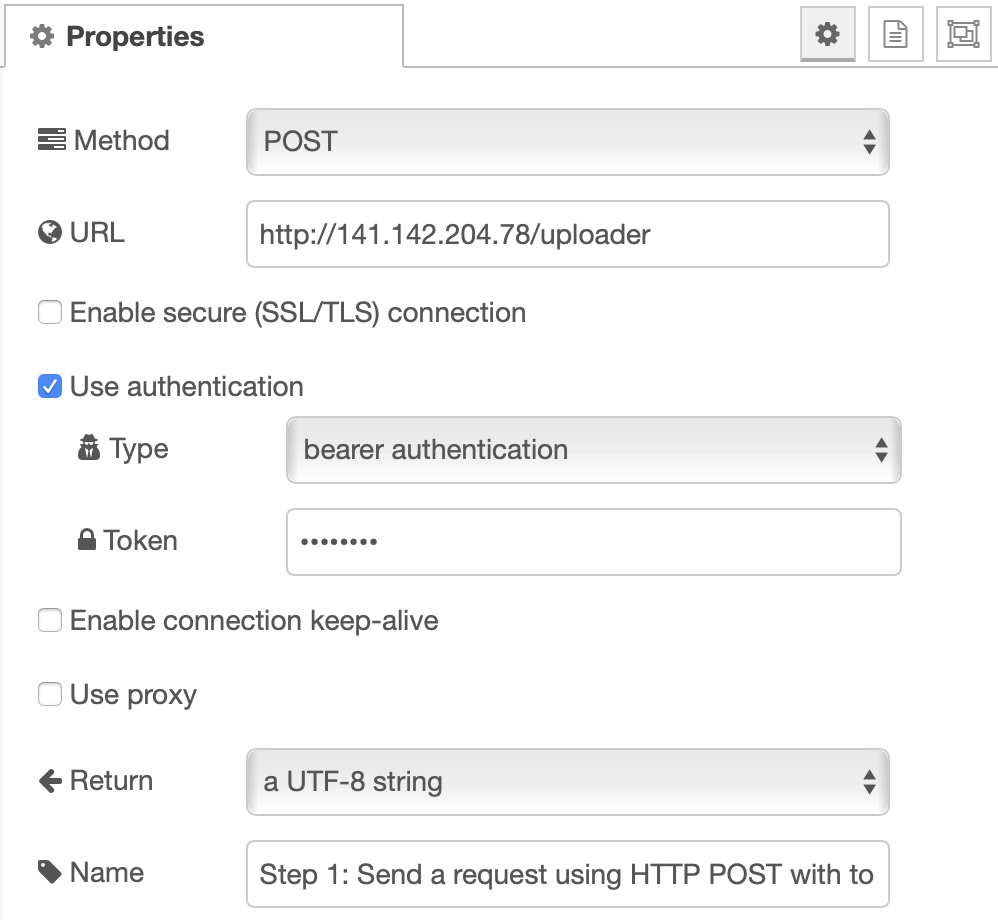
\includegraphics[width=12cm]{2_2.png}
\end{center}
a \textit{function} node which gets the taskID,
\begin{center}
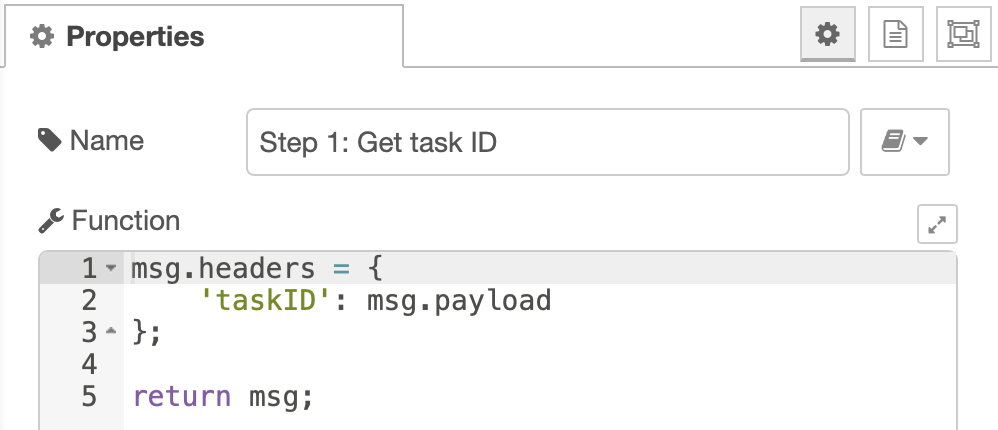
\includegraphics[width=12cm]{2_3.png}
\end{center}
and a \textit{debug} node which shows the taskID.
\item \textbf{Step 2 \& Step 3}
\begin{center}
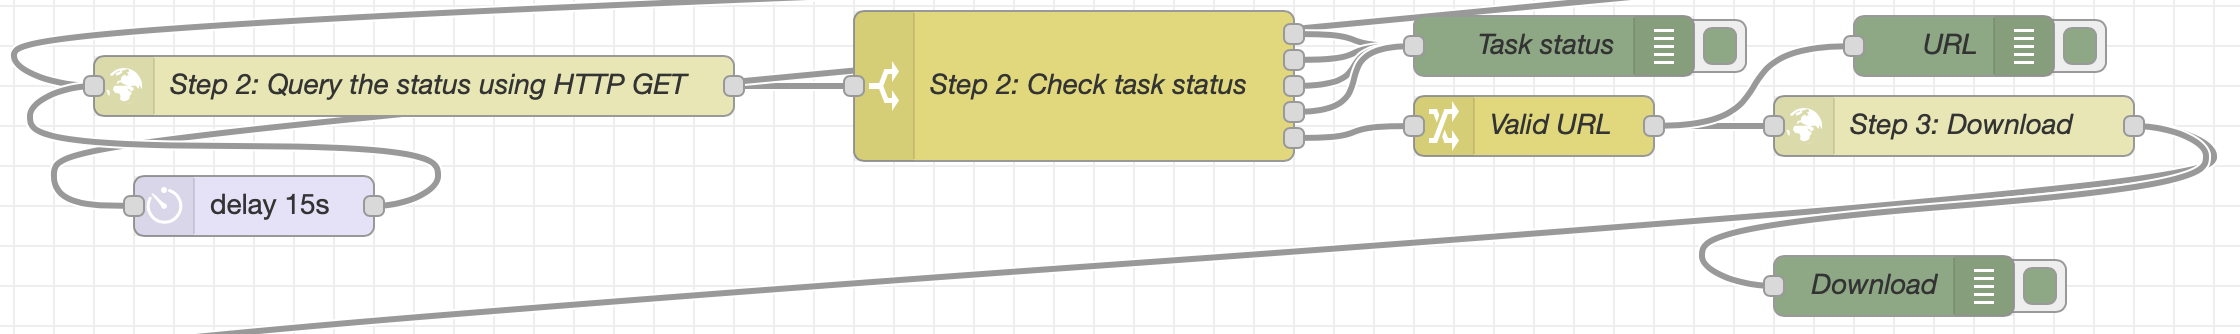
\includegraphics[width=12cm]{3.png}
\end{center}
There are 8 nodes in this group, including an \textit{HTTP request} node which queries the task status,
\begin{center}
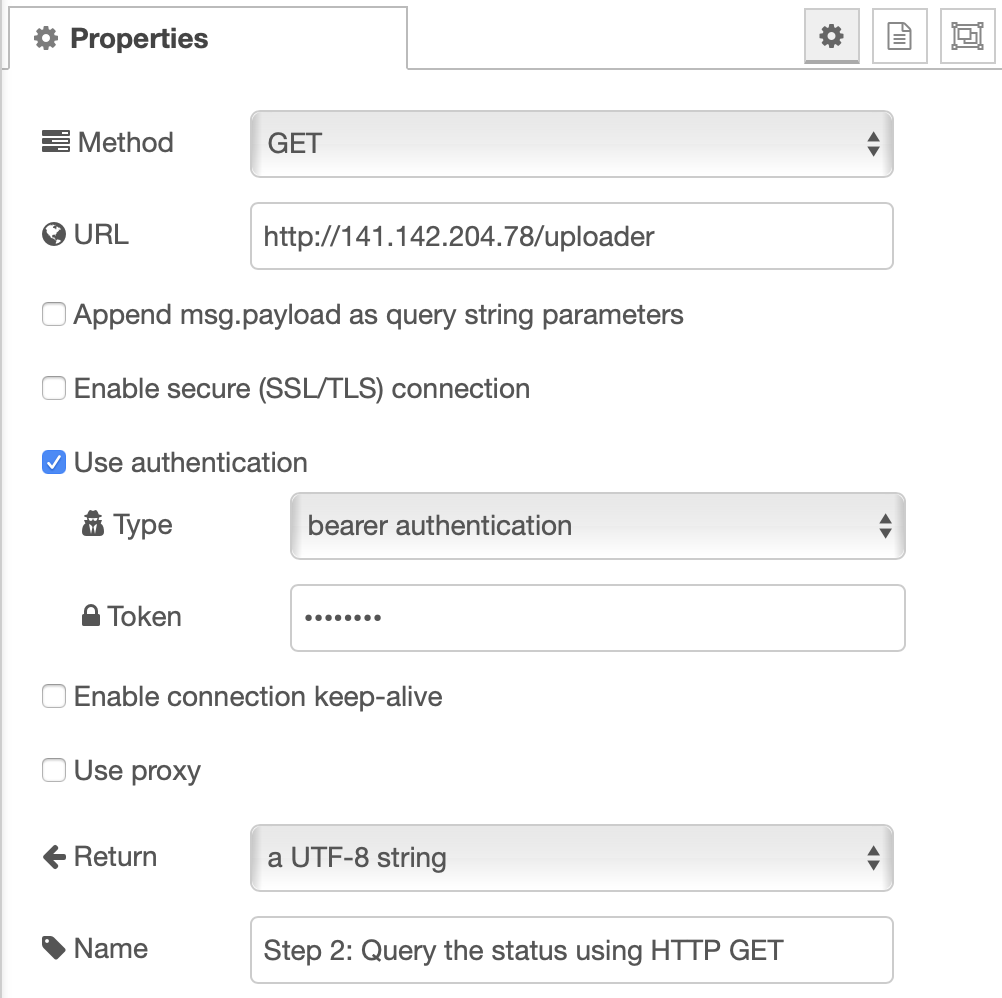
\includegraphics[width=12cm]{3_1.png}
\end{center}
a \textit{switch} node which handles different task statuses,
\begin{center}
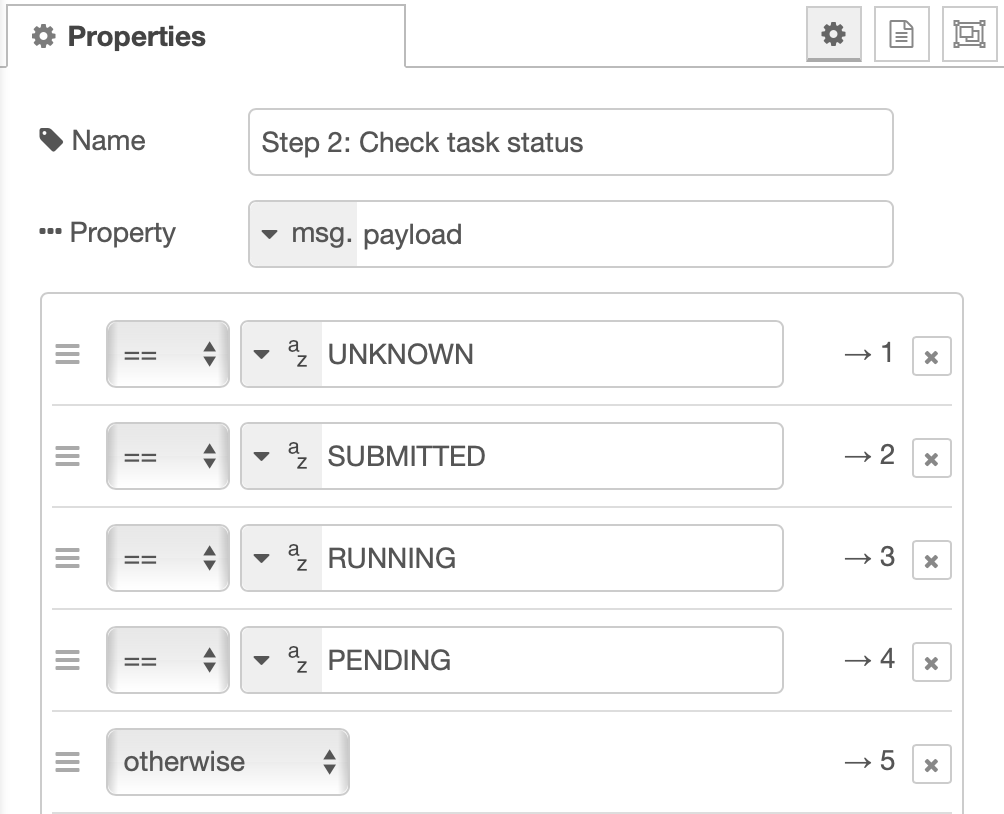
\includegraphics[width=12cm]{3_2.png}
\end{center}
a \textit{change} node which gets the URL,
\begin{center}
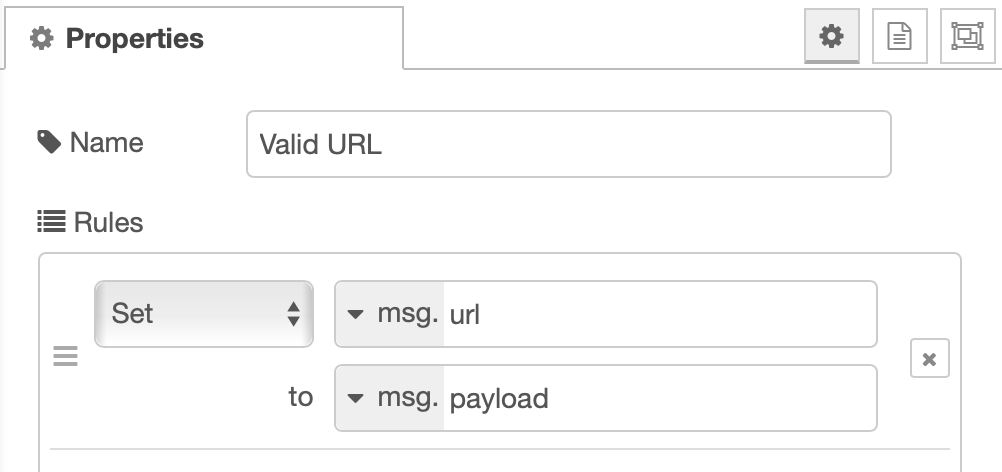
\includegraphics[width=12cm]{3_3.png}
\end{center}
an \textit{HTTP request} node which sends a request to download the feedback,
\begin{center}
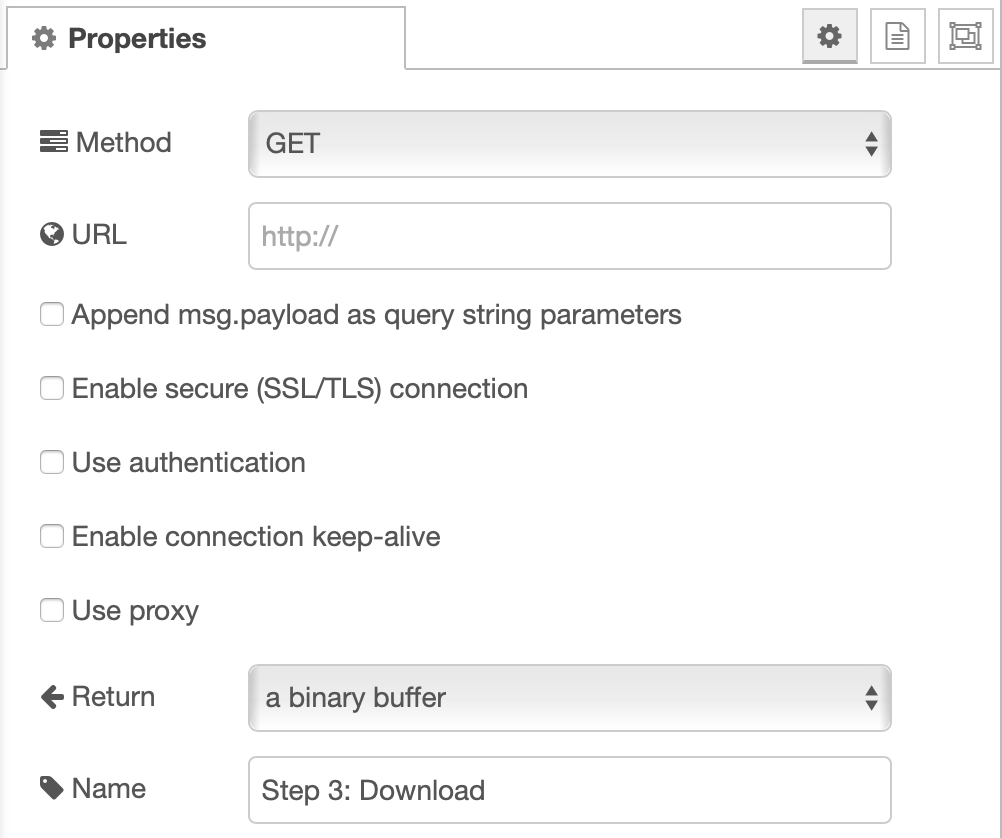
\includegraphics[width=12cm]{3_4.png}
\end{center}
and some \textit{debug} nodes that show task status, URL, and download information.
\item \textbf{Step 4}
\begin{center}
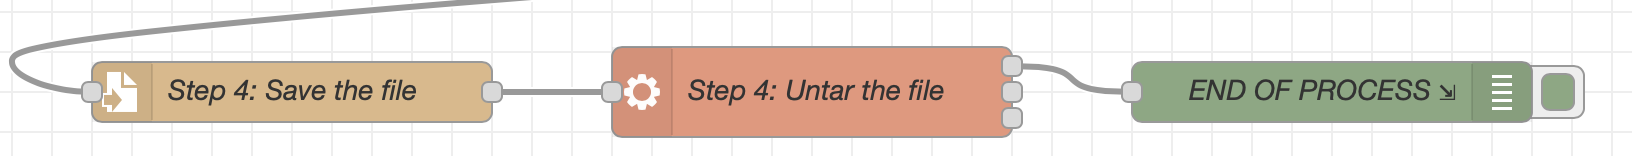
\includegraphics[width=10cm]{4.png}
\end{center}
There are 3 nodes in this group, including a \textit{file in} node which saves the feedback,
\begin{center}
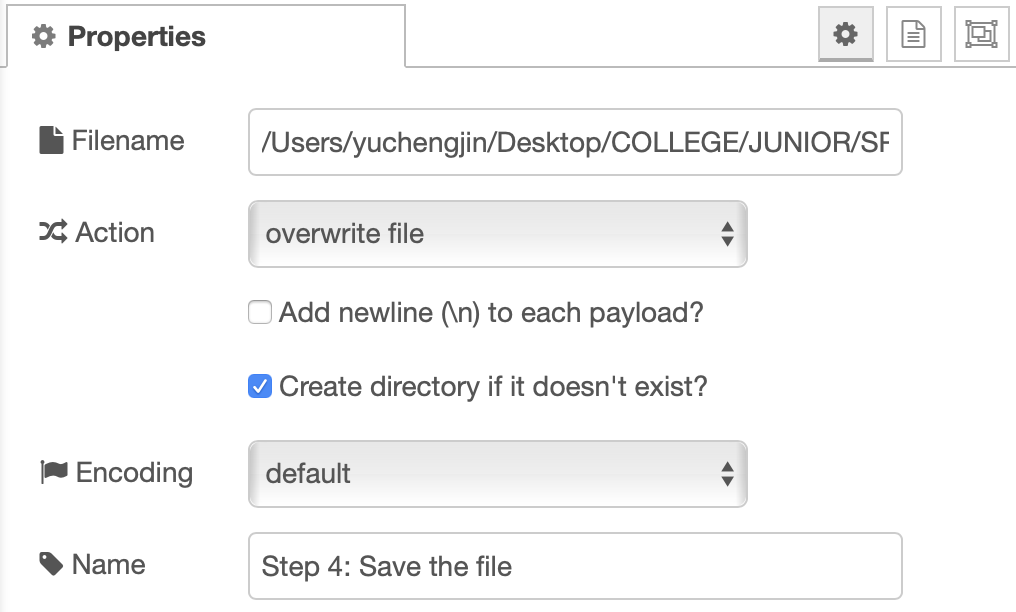
\includegraphics[width=12cm]{4_1.png}
\end{center}
an \textit{exec} node which untars the file,
\begin{center}
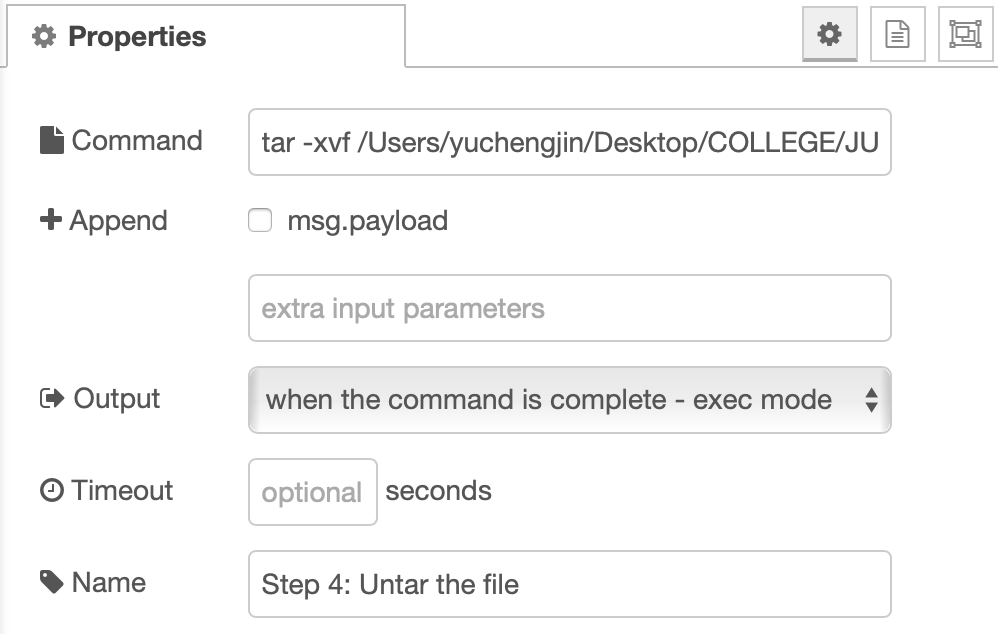
\includegraphics[width=12cm]{4_2.png}
\end{center}
and a \textit{debug} node which shows the message that the process is finished.
\item \textbf{Catch}
\begin{center}
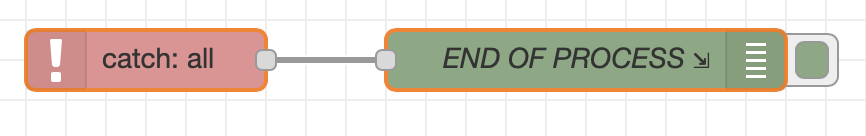
\includegraphics[width=10cm]{5.png}
\end{center}
This group handles with errors.
\end{itemize}
\subsection{Check Point III}
\textbf{[2 pts]} Describe at least three challenges you encountered during the development of the Node-RED flow in Part I and how you resolved them.
\begin{itemize}
\item Because \textit{function} nodes use JavaScript to specify their functionalities, but we had not learned JavaScript before Lab 2. Therefore, we had to study basic knowledge about JavaScript, and by searching online materials, we successfully learned how to change massage header and payload, then finally finished choosing the correct data type, device type, task type, etc.
\item At first we did not know how to repeatedly query the task status, and tried several unsuccessful methods. By asking questions in Piazza, we learned that by adding a \textit{delay} node, we could realize the functionality of repeatedly querying the task status.
\item For the last step, downloading and untaring the file, we first ended up with damaged file. And we carefully examined every parameter and finally found that we should save a binary buffer instead of an UTF-8 string.
\end{itemize}
\pagebreak
\section{Part II}
\subsection{Check Point I} 
\textbf{[1 pts]} Collect and report the execution time of all datasets with a table, for basic and tiled MM on both V100 and TX2.
\begin{center}
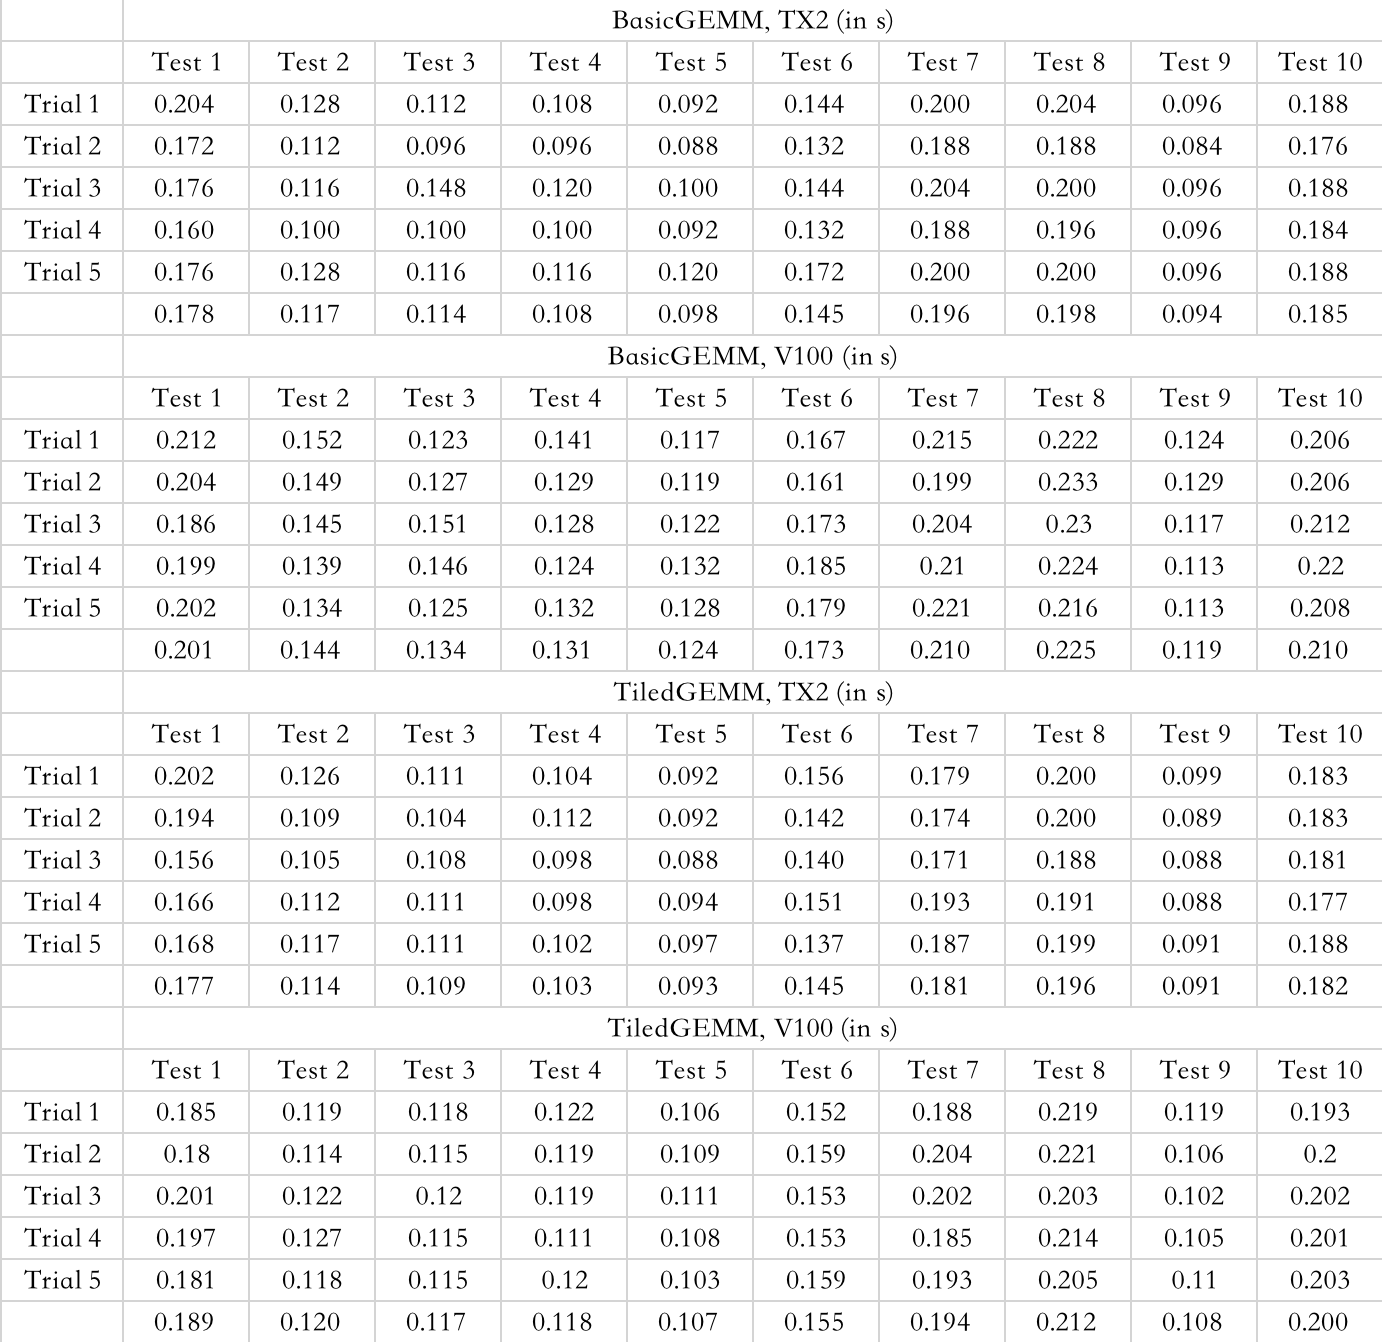
\includegraphics[width=15cm]{time.png}
\end{center}
Above is our table. For BasicGEMM on TX2, BasicGEMM on V100, TiledGEMM on TX2, and TiledGEMM on V100, we each ran 5 times. 
\pagebreak
\subsection{Check Point II}
\textbf{[2 pts]} Compare the execution time and explain how TiledGEMM can reduce global memory access. Calculate and report the maximum theoretical reduction of global memory access with your implementation.
\begin{itemize}
\item \textbf{Compare the execution time}: from the table above, TiledGEMM runs faster than BasicGEMM, and they both run faster on TX2 compared to V100.
\item \textbf{How TiledGEMM can reduce global memory access}: TiledGEMM takes the advantage of shared memory. For each tile, Tiled MM copies data from global memory to shared memory and then performs calculations. For global memory, it takes around 500 cycles to access data; but for shared memory, it takes only about 5 cycles to access data. Although it takes some time to copy data from global memory to shared memory, but for each calculation shared memory reduces the number of cycles to access data, so TiledGEMM overall decreases the execution time by reducing global memory access.
\item \textbf{Calculate and report the maximum theoretical reduction of global memory access}: using 16x16 tiling, we reduce the global memory access by a factor of 16; using 32x32 tiling, we reduce the global memory access by a factor of 32; generally, using $N \times N$ tiling, we reduce the global memory access by a factor of $N$. It's easy to come up with the conclusion, just think about the multiplication of two $N \times N$ matrices, if we use BasicGEMM, it will access global memory $2 \times N \times N \times N$ times; but for TiledGEMM, using $N \times N$ tiling, it will access global memory $2 \times N \times N$ times, so \textbf{using $N \times N$ tiling, we reduce the global memory access by a factor of $N$}.
\end{itemize}
\subsection{Check Point III}
\textbf{[2 pts]} Compare the hardware specifications of V100 and TX2 (e.g. number of SMs, etc.) and briefly explain the factors that causes the performance diference.
\begin{center}
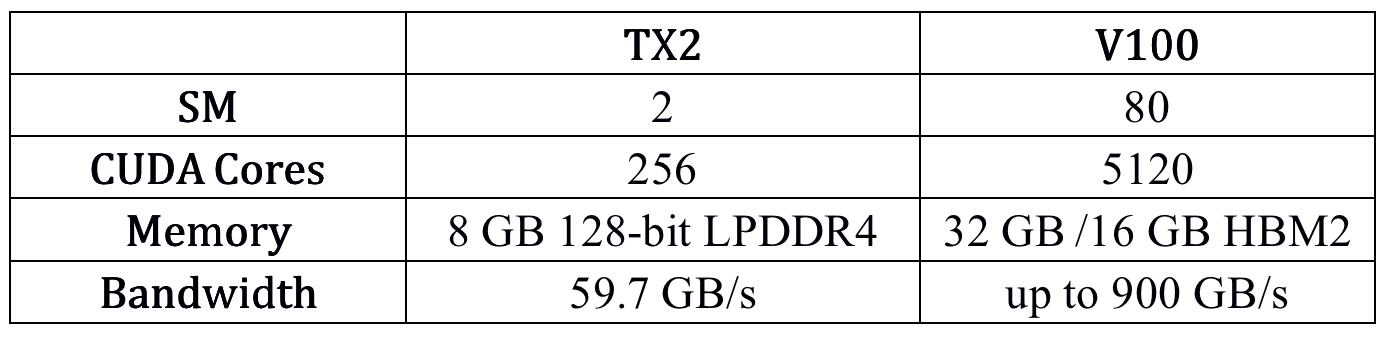
\includegraphics[width=12.5cm]{data.png}
\end{center}
Above table shows the the hardware specifications of V100 and TX2\footnote{Data from NVIDIA official datasheet, https://www.nvidia.com/en-us/data-center/v100, https://developer.nvidia.com/embedded/jetson-tx2.}.\\
\\ From the hardware specifications we know that compared with TX2, V100 has more SMs and CUDA cores, larger memory and bandwidth. With more SMs and CUDA cores, V100 is able to process tasks at a higher speed; and with larger memory and bandwidth, V100 is able to handle more data and has a significantly higher throughput. So in theory, V100 generally performs better than TX2. But since the matrix multiplication task in our Lab 2 maybe too easy, thus the full resources of V100 were not being taken advantage of, so we did not see V100 outperform this time.

\end{document}

%% 
%% This work consists of these files mcmthesis.dtx,
%%                                   figures/ and
%%                                   code/,
%% and the derived files             mcmthesis.cls,
%%                                   mcmthesis-demo.tex,
%%                                   README,
%%                                   LICENSE,
%%                                   mcmthesis.pdf and
%%                                   mcmthesis-demo.pdf.
%%
%% End of file `mcmthesis-demo.tex'.
